\chapter{Inverter power consumption}

\section{Dynamic power consumtion}
Only in case of charge of a capacitance so in a LOW to HIGH transition at the output of an inverter. \\
The most general formula for the power dissipated in this process is
\begin{equation}
P_{dyn}=C_LV_{DD}^2f_{1\rightarrow 0}
\end{equation}
where $f_{1\rightarrow 0}$ is the frequency of the 0-1 transition at the output node. This term can be deconposed in 2 factor the clock of the circuit and the switching activity $\alpha_{SW}$ that is the probability to have a transition from 0 to 1 at the output.\\
\vspace{2mm}
\tab In case of a square wave we have 
\begin{equation}
f_{1\rightarrow 0}=f_{clk}\cdot \alpha_{SW}=f_{clk}\cdot \frac{1}{2}
\end{equation}
\tab In case of a randoom signal 
\begin{equation}
f_{1\rightarrow 0}=f_{clk}\cdot \alpha_{SW}=f_{clk}\cdot \frac{1}{4}
\end{equation}
\vspace{5mm}
In the end we can write this 2 final equation for dynamic power dissipation
\begin{equation}
P_{dyn}=C_LV_{DD}^2 f_{clk}\cdot \alpha_{SW}
\end{equation}
\begin{equation}
E_{dyn}=C_LV_{DD}^2\alpha_{SW}
\end{equation}
In case of a chain of inverters $C_L$ is the sum of all the capacitance at the output nodes of the single inverters.\\

\section{Cross-conduction power consumption}
Due to the finite slope of the input signal there is a finite time when both p-mos and -mos are on creating a low impedance path between $V_{DD}$ and GND.\\

\centering
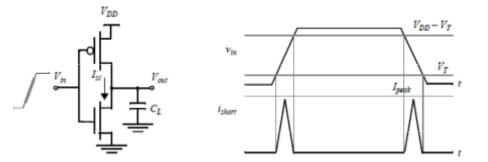
\includegraphics[width=0.7\textwidth]{C4_1.png}\\
\raggedright

\centering
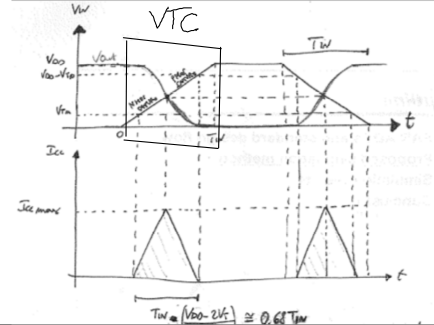
\includegraphics[width=0.5\textwidth]{C4_1b.png}\\
\raggedright

Defining $T_{in}$ as the time needed by the input signal to transition from GND to $V_{DD}$ and vice-versa and $I_{peak}$ the velocity saturation current of the n-mos (when the input and the output are at $V_m$) we can compute the cross-conduction energy as (assuming $V_{tp}=V_{tn}$) 
\begin{equation}
E_{cc}= \frac{1}{2} V_{DD}I_{peak}\cdot 0.68 \cdot T_{in}
\end{equation}
If we consider an input signal with an update frequency of f with continuos switch HL LH the power is 
\begin{equation}
P_{cc}=\frac{V_{DD}I_{peak} \cdot 0.68 \cdot T_{in}}{2} f
\end{equation}

\vspace{5mm}

With capacitve loads the cross-conduction power becomes smaller than without.\\ 
The cross conduction power can be neglected when 
\begin{equation}
T_{in}<10\tau_p
\end{equation}
with $\tau_p$ propagation delay of the stage.\\


\section{Static power consumption}
It's due to the subthreshold current of the MOS devices.

